\begin{figure*}[h]                                                           
 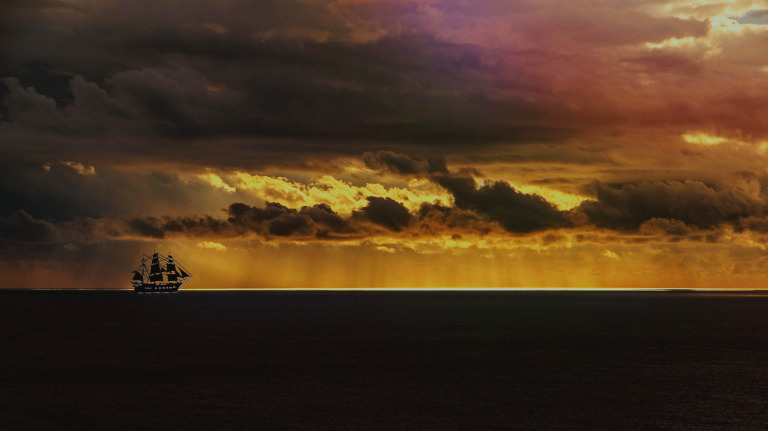
\includegraphics[width=\linewidth]{./media/images/boat}%
  \small{\textsc{\\ Peter M.J. Gross's} editing made this issue of
    \textsc{Discoverer's Digest} a much better work than it otherwise would be;
    he helped navigate my way to publishing this issue.}
  \label{fig:boat}%                                                 
\end{figure*}                                                                
\begin{quotation} 
\noindent\color{Sepia}{\small{\textit{\textbf{“Talent is a flame. Genius is
        a fire.” }}}}\\[2mm]
   \hfill\color{Sepia}{\scriptsize{\textendash Bernard Williams}}
\end{quotation} 

\section{peter m.j. gross: they don't come better}
\lettrine[lines=3]{\color{BrickRed}I}{\enspace} want to thank \textit{Peter M.J. Gross} for his fantastic work editing this
edition. To give the credit he deserves will sound trite and woefully inadequate
at the same time. Peter is a man who's thoroughness, understanding, and
relentless pursuit of quality are second to none.

By the way, Peter doesn't know I'm writing this \textit{thanks} here so if there are any
errors or awkward grammar the fault is fully my own.

\noindent Thank you, Peter.


\section{coming up}
The next issue of \textit{Discoverer's Digest} covers the results of this year's
\textsc{IF Comp} results and possibly an interview from one or two of the authors.

Covered also will be more mapping techniques and a guide for
\textsc{gps}\textendash enabled \textsc{if}.

See you next time! \\ \\

\noindent Fair Winds, \\ \\

\noindent\textsc{\href{mailto:cooper@discdigest.xyz}{D. Cooper Stevenson}}



%\noindent \href{mailto:cooper@cooper.stevenson.name}{\textsc{D. Cooper Stevenson}} 

